

\chapter{Vorticity}

A view of Jupiter's swirly atmosphere, or following the motion of
hurricanes on Earth, or simply the whirpools in a stream \figp{fig:vortices}, will suffice
to convince you that {\it vortices} are structures that form in flows
and that behave in an independent way than the rest of the
fluid. They're advected by the flow and seem frozen into the fluid as
it flows. 

To understand this behavior, let us define the concept of {\it
  vorticity}. Vorticity is the curl of the velocity

\beq
\v{\omega} = \curl{\v{u}}
\eeq

Indeed, under some conditions (that are often realized in nature), we
will show that vorticity is {\it conserved}. 

\section{Vorticity equation}

\begin{figure}
  \begin{center}
    \resizebox{\textwidth}{!}{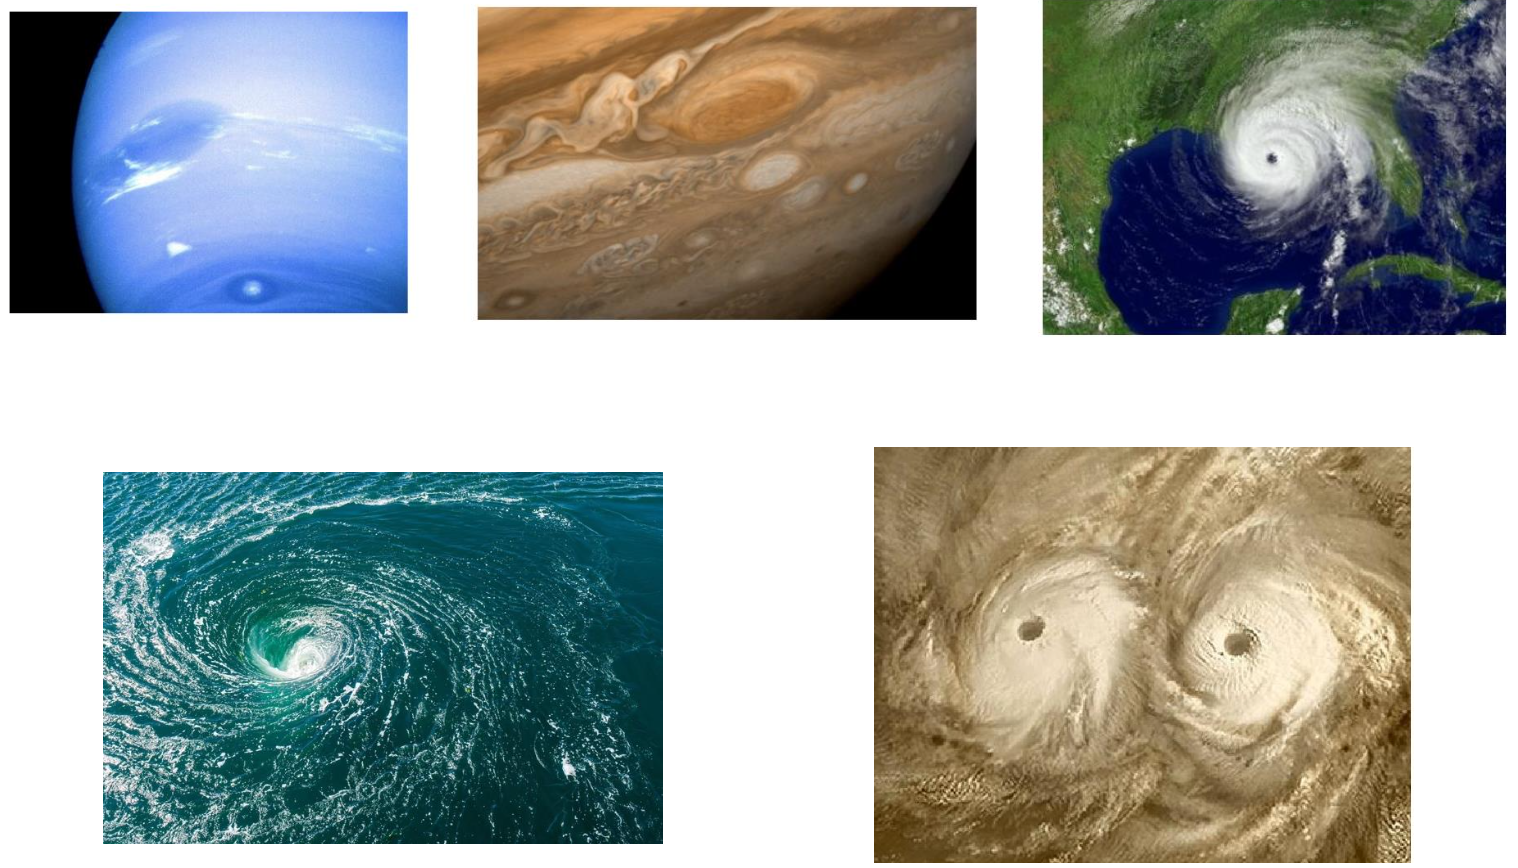
\includegraphics{./figs/vortices.png}}
  \end{center}
  \caption[]{Vortices: an ubiquitous fluid mechanics phenomenon.}
  \label{fig:vortices}
\end{figure}

If we take the Navier-Stokes equation and curl it

\beq
\frac{\partial \v{\omega}}{\partial t} = -\curl{\left[\left(\v{u}\cdot\del\right)\v{u}\right]}
-\curl{\left(\frac{1}{\rho}\grad{p}\right)} + \curl{\v{f}} + \nu\Laplace\v{\omega}
\eeq

Let us examine the terms. Body forces like gravity are usually conservative, so we set
$\curl{\v{f}}=0$. The curl of the pressure gradient is 

\beq
\curl{\left(\frac{1}{\rho}\grad{p}\right)} =-\frac{1}{\rho^2}\grad{\rho} \times \grad{p}
\eeq

to take the curl of the inertial term we transform 

\beqn
\left(\v{u}\cdot\del\right)\v{u} &=& \frac{1}{2}\grad{u^2} -\v{u}\times\left(\curl{\v{u}}\right)\\
&=&\frac{1}{2}\grad{u^2} -\v{u}\times\v{\omega}
\eeqn

when taking the curl of it, the first term cancels, so we're left with 

\beq
\frac{\partial \v{\omega}}{\partial t} = \curl{\left(\v{u}\times\v{\omega}\right)}
+\frac{1}{\rho^2}\grad{\rho} \times \grad{p} + \nu\Laplace{\v{\omega}}
\label{eq:vort-baro-diff}
\eeq

The curl of the vector product is

\beqn
\curl{\left(\v{u}\times\v{\omega}\right)} &=&\varepsilon_{ijk}\varepsilon_{kpq}\partial_ju_p\omega_q\\
&=&\left(\delta_{ip}\delta_{jq}-\delta_{iq}\delta_{jp}\right)\partial_ju_p\omega_q\\
&=&\partial_ju_i\omega_j - \partial_ju_j\omega_i\\
&=&u_i\partial_j\omega_j +\omega_j\partial_ju_i - u_j\partial_j\omega_i-\omega_i\partial_ju_j\\
&=&\v{u}\left(\Div{\v{\omega}}\right) + \left(\v{\omega}\cdot\del\right) \v{u} -\left(\v{u}\cdot\del\right)\v{\omega} -  \v{\omega}\left(\Div{\v{u}}\right)
\eeqn

Since vorticity is a curl, the first time cancels. What is left yields
the vorticity equation 

\beq
\boxed{
\frac{\partial \v{\omega}}{\partial t} =
-\left(\v{u}\cdot\del\right)\v{\omega}  -
\v{\omega}\left(\Div{\v{u}}\right) + \left(\v{\omega}\cdot\del\right) \v{u} 
+\frac{1}{\rho^2}\grad{\rho} \times \grad{p} + \nu\Laplace{\v{\omega}}
}
\eeq

Let us understand this equation. The first term in the RHS is an
advection term. The second is a compression term. The 3rd term is
stretching, the fourth is the only source term, the baroclinic
term. The last one is diffusion. 

The advection shows that vorticity is advected by the flow, like the
other quantities, so we can write a Langrangian formulation

\beq
\frac{D \v{\omega}}{D t} =- \v{\omega}\left(\Div{\v{u}}\right) +
\left(\v{\omega}\cdot\del\right) \v{u}  +\frac{1}{\rho^2}\grad{\rho} \times \grad{p} + \nu\Laplace{\v{\omega}}
\eeq

The compression term shows that a vortex is amplified if the
flow is compressed, and weakened if the flow expands. Since vorticity
is the fluid circulation, we expect that this is a result of
conservation of angular momentum. 

\subsection{The baroclinic term}

A barotropic fluid has $p = p(\rho)$. The surfaces of constant
pressure and constant density are aligned, so the
gradients point in the same direction.
The word barotropic comes from baro (pressure) + tropos
(direction). Meaning pressure gradient is in the same
direction as the density gradient.

A baroclinic fluid has $p = p(\rho,T)$. The surfaces of constant
pressure and constant density can be inclined, with the
gradients pointing in different directions.
The word baroclinic comes from baro (pressure) +
inclination (direction). Meaning pressure and density
gradients are misaligned.

Notice that the polytropic equation of state $p = K \rho^\gamma$ is barotropic.
The interior of stars and giant planets are well-approximated by
polytropes. Notice also that $K=p/\rho^\gamma$ is the entropy. This
means that for barotropic fluids, the entropy is constant.
The condition of baroclinicity then translates simply into: {\it varying entropy}.
An entropy gradient leads to vortex generation by convection \figp{fig:baroclinic}.


\begin{figure}
  \begin{center}
    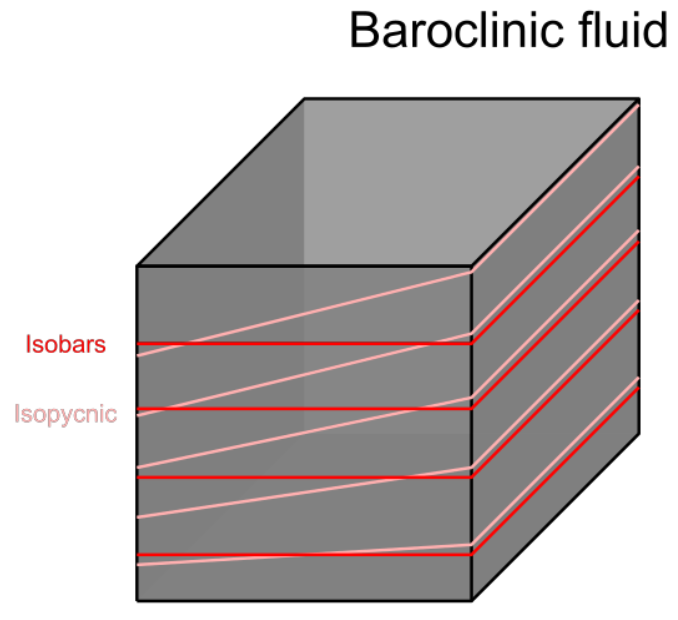
\includegraphics[height=.45\linewidth]{./figs/baroclinicfluid.png}
    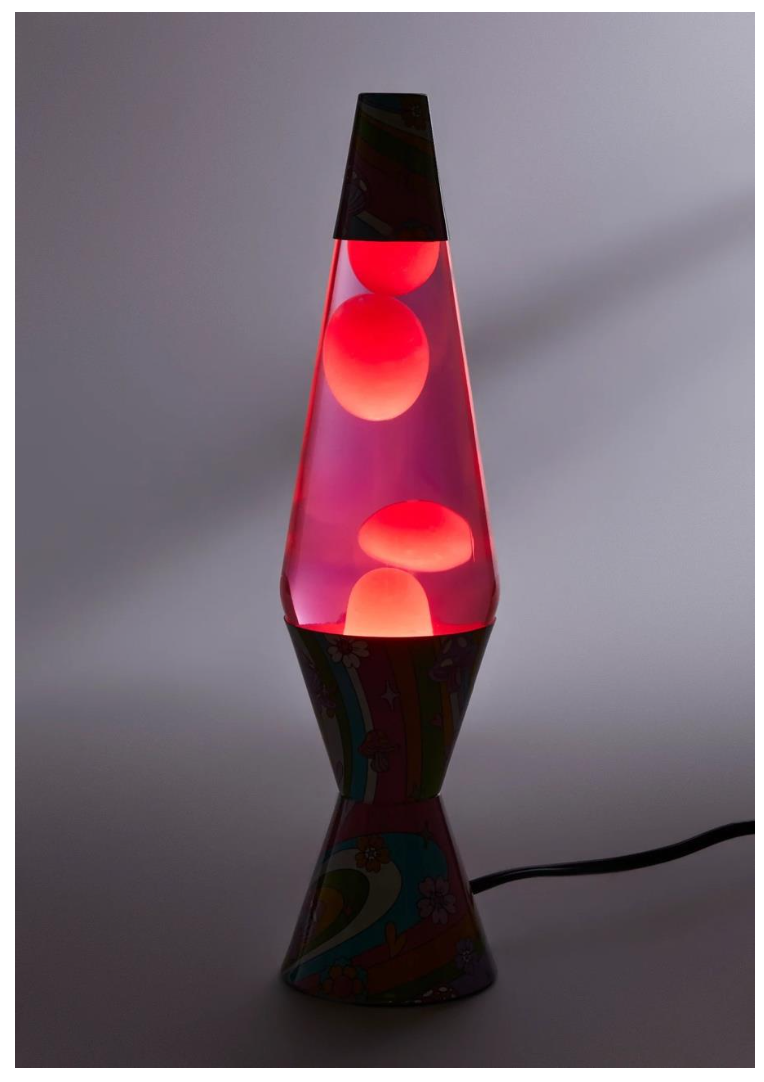
\includegraphics[height=.45\linewidth]{./figs/lavalamp.png} 
%    \resizebox{.47\textwidth}{!}{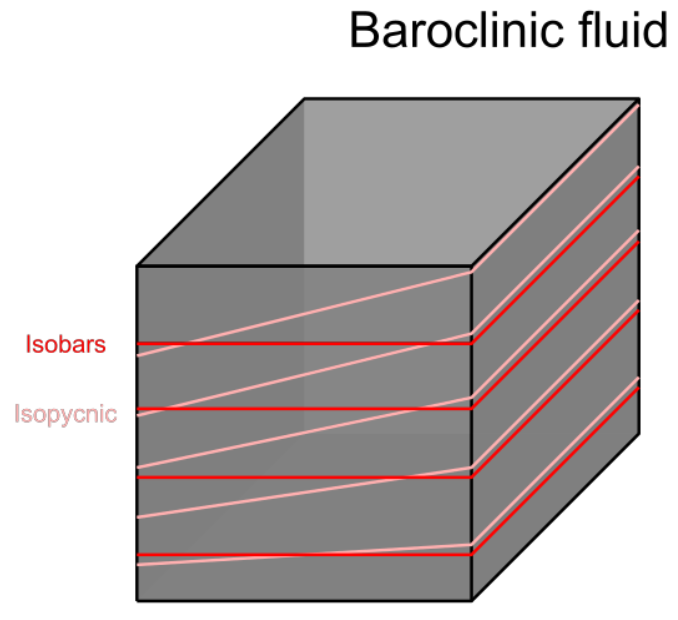
\includegraphics{./figs/baroclinicfluid.png}}
 %   \resizebox{.47\textwidth}{!}{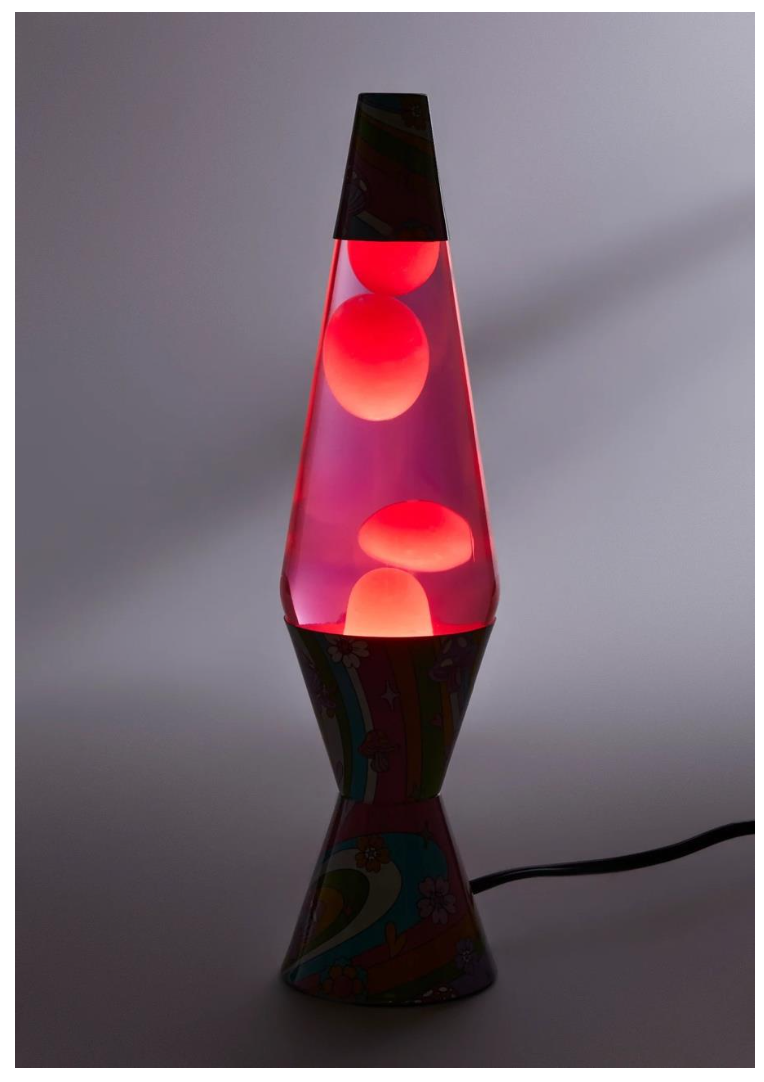
\includegraphics{./figs/lavalamp.png}}
  \end{center}
  \caption[]{Baroclinic fluids: inclined surfaces of constant density
    and constant pressure, i.e., a non-zero
    $\grad{p}\times\grad{\rho}$ is the source of
    vorticity. Alternatively, one can thing of an entropy gradient
    sourcing vorticity, as in convection in a lava lamp.}
  \label{fig:baroclinic}
\end{figure}


\subsection{The stretching term}

Let's verify what the strectching term does and why it is called
so. Consider the flow in \fig{fig:stretching}. The velocity points
only in the x-direction, but with a gradient in the y-direction, i.e.,
it has shear. As as
result, it will advect the y-pointing vorticity bundle in a {\it differential}
way. The vorticity at a time in the future will be pointing
diagonally. We started with a vorticity purely in the y-direction, but
a component was built in the x-direction, the direction of the
flow. It was {\it stretched} in the direction of the sheared
flow. Stretching is essentially a sheared advection, changing the
shape of the function, something the advection alone cannot do. It
stretches the vorticity $\v{\omega}$ when the velocity is shearing
in the direction parallel to $\v{\omega}$. Hence its form
$\left(\v{\omega}\cdot\del\right) \v{u}$. 

\begin{figure}
  \begin{center}
    \resizebox{\textwidth}{!}{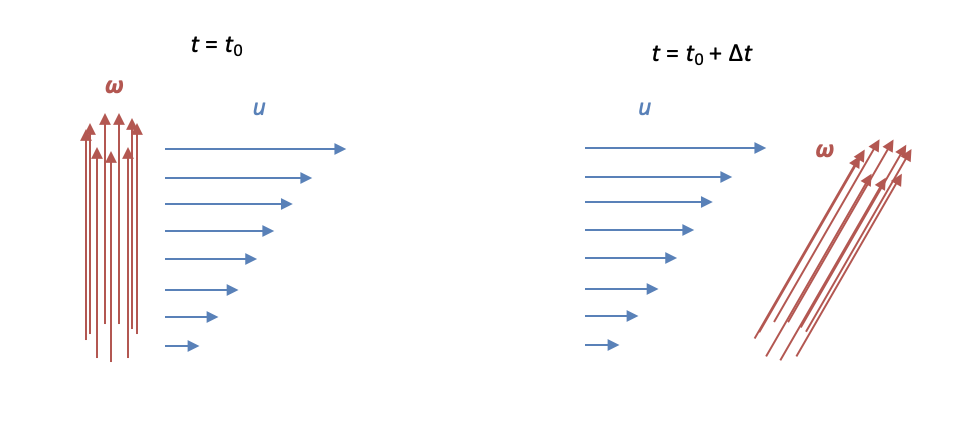
\includegraphics{./figs/stretching.jpg}}
  \end{center}
  \caption[]{Vorticity is amplified in the direction of shear. The
    term responsible for this behavior is the stretching term $\left(\v{\omega}\cdot\del\right)\v{u}$.}
  \label{fig:stretching}
\end{figure}

Notice that if the flow is 2D, there is no stretching, as the
vorticity is perpendicular to the flow, canceling
$\omega_j\partial_j$ \figp{fig:stretching2D}. If on top of that we consider that the flow is
imcompressible, of high Reynolds number, and ignore the baroclinic
term, then vorticity is conserved. 

\beq
\frac{D \v{\omega}}{D t}=0 
\eeq

That vorticity is conserved in this flow explains why vortices are
persistent structures. 

\begin{figure}
  \begin{center}
    \resizebox{.6\textwidth}{!}{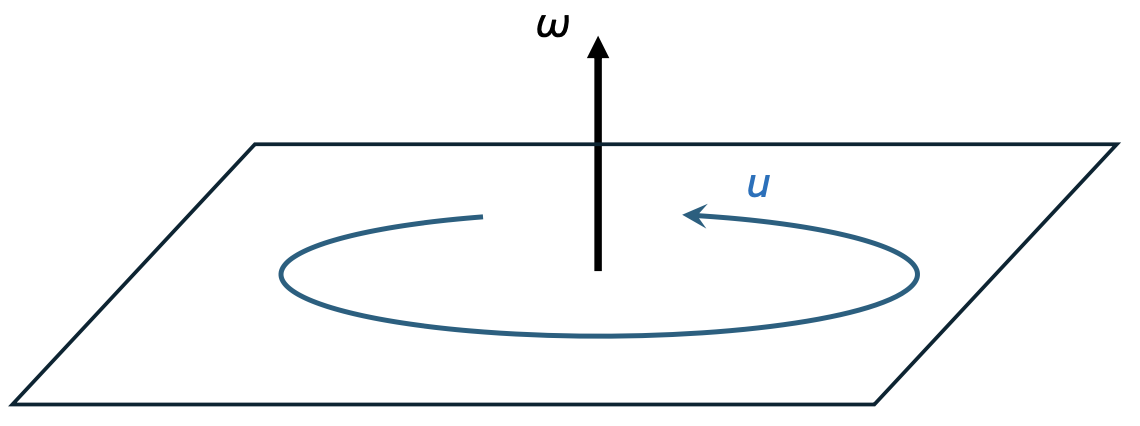
\includegraphics{./figs/stretching2D.png}}
  \end{center}
  \caption[]{If the motion is restricted to a plane, then the
    vorticity is always out of the plane, and the stretching term is zero.}
  \label{fig:stretching2D}
\end{figure}

\section{Kelvin vorticity theorem} 

%VonKarmanStreet.png
%DalembertParadox.png

\begin{figure}
  \begin{center}
    \resizebox{\textwidth}{!}{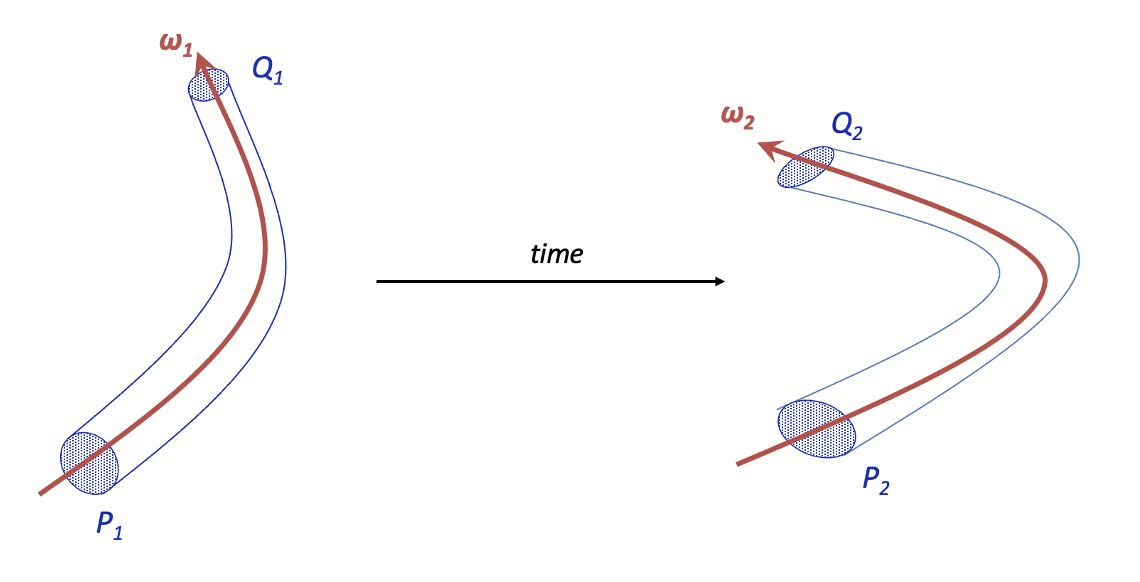
\includegraphics{./figs/KelvinFluxFreezing.png}}
  \end{center}
  \caption[]{Kelvin flux-freezing theorem. Two patches connected by a
    vortex line will remain connected by the same vortex line at
  all times. Irrespective of advection, stretching, and compression,
  the topology of a vortex line is conserved. The vortex is ``frozen''
  on the fluid.}
  \label{fig:KelvinFluxFreezing}
\end{figure}


\begin{figure}
  \begin{center}
    \resizebox{.75\textwidth}{!}{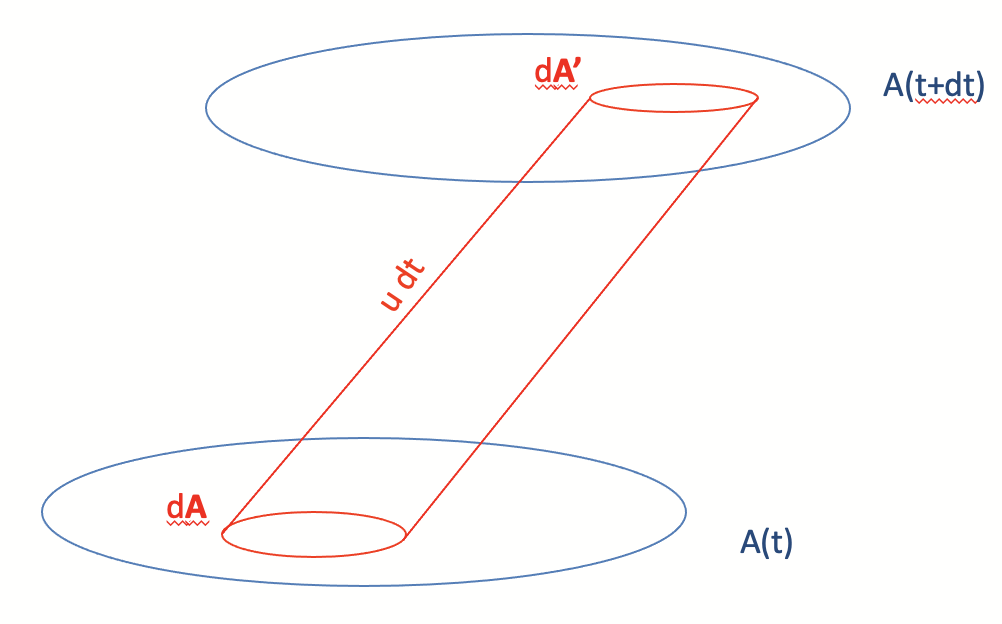
\includegraphics{./figs/KelvinTheorem_Cylinder.png}}
  \end{center}
  \caption[]{A patch $d\v{A}$ flows with velocity $\v{u}$ and is deformed into $d\v{A}^\prime$ within
    a time interval $dt$. This describes a cylinder as given above.}
  \label{fig:KelvinTheorem_Cylinder}
\end{figure}

According to \eq{eq:vort-baro-diff}, a barotropic flow at high
Reynolds numbers satisfies

\beq
\frac{\partial \v{\omega}}{\partial t} = \curl{\left(\v{u}\times\v{\omega}\right)}
\eeq

This equation implies that the flux of vorticity is conserved, and the
vortex lines move with the fluid. This is why we can visualize the
vortices as entities embedded in the fluid:  the vortex lines are ``frozen'' into the
fluid, and move with the flow. This is known as {\it Kelvin's vorticity
theorem} or Kelvin's {\it flux-freezing} theorem. 

The theorem states that

\beq
\frac{d}{dt}\int_A \v{\omega} \cdot d\v{A}  = 0 
\eeq

in plain words, in means that if you consider a surface $A$ inside a
fluid at a given time, the flux of vorticity through this surface is
unchanged as the surface evolves due to whatever motion happens in the fluid.

The consequences of this theorem are remarkable. Once two surface
elements are connected by a vortex line, they will remain so. The
vortex is frozen-in and moves with the fluid \figp{fig:KelvinFluxFreezing}. 

The surface elements $P$ and $Q$ change into $P^\prime$ and $Q^\prime$ as a
result of fluid motions. Due to flux-freezing, the vortex line that
connects $P$ and $Q$ will also connect $P^\prime$ and $Q^\prime$ and
the vortex topology is preserved. This gives a neat visualization of
the vortices: as we can guess the vorticity configuration if we know the
fluid flow. The vortex is an almost material, plastic substance that
moves with the flow. 

Proof:

Kelvin's theorem applies to any vector that satisfies

\beq
\frac{\partial \v{Q}}{\partial t} = \curl{\left(\v{u}\times\v{Q}\right)}
\label{eq:kelvin1}
\eeq

to show that, we need to show that \eq{eq:kelvin1} is equivalent to 

\beq
\frac{d}{dt}\int_A \v{Q} \cdot d\v{A}  = 0 
\eeq

we apply Leibniz rule of derivating under the integral to 

\beq
\frac{d}{dt}\int_A \v{Q} \cdot d\v{A} = \int \frac{\partial
  \v{Q}}{\partial t} dA + \v{Q}\cdot\frac{d}{dt}\left(d\v{A}\right)
\label{eq:kelvin-leib}
\eeq

the term $\frac{d}{dt}\left(d\v{A}\right)$ is the time variation of
a surface element $d\v{A}$. The area $A$ in time $t$ goes to $A^\prime$
in time $t+dt$ \figp{fig:KelvinTheorem_Cylinder}. 


\beq
\frac{d}{dt}\left(d\v{A}\right)  = {\rm lim}_{\Delta t\rightarrow 0}
\frac{d\v{A}^\prime - d\v{A}}{\Delta t}
\eeq

how do we find $d\v{A}^\prime - d\v{A}$?

The vector area integral over a closed surface is zero: $\oint d\v{A}
= 0$. \classcomm{give cube as example}. So let's close the surface  \figp{fig:KelvinTheorem_Cylinder}

The side area is $dS = \oint dl \times \v{u}dt$, so the total area of the
cylinder is

\beq
d\v{A}^\prime -d\v{A} + \oint dl \times \v{u}dt = 0
\eeq

reversing the cross product 

\beq
d\v{A}^\prime -d\v{A} = dt\oint \v{u} \times dl = 0
\eeq

it then follows that

\beq
\frac{d}{dt}\left(d\v{A}\right)  = {\rm lim}_{\Delta t\rightarrow 0}
\frac{d\v{A}^\prime - d\v{A}}{\Delta t} = \oint \v{u} \times dl
\eeq

So the last term of \eq{eq:kelvin-leib} is

\beq
\int_A \v{Q}\cdot \frac{d}{dt}\left(d\v{A}\right) = \int_A \oint \v{Q}\cdot\left(\v{u} \times dl\right)
\eeq

and because 

\beq
\v{A} \cdot \left(\v{B} \times \v{C}\right) = \v{B} \cdot \left(\v{C} \times \v{A} \right)= \v{C} \cdot \left(\v{A} \times \v{B}\right)
\eeq

we can write 

\beq
\int_A \v{Q}\cdot \frac{d}{dt}\left(d\v{A}\right) = \int_A \oint \left(\v{Q}\times\v{u} \right)\cdot dl
\eeq

This is a strange integral. It represents the sum over all little
$d\v{l}$ elements that are 
embedded in the area A. We need to do the line integrals over all the
surface elements that compose A. Because the internal line integrals
cancel out \classcomm{show example of honeycomb pattern} this reduces
to an integral over the contour C of S.

\beq
\int_A \oint \left(\v{Q}\times\v{u} \right)\cdot dl = \oint_C
\left(\v{Q}\times\v{u} \right) dl 
\eeq

which, by Stokes theorem, is

\beq
\oint_C \left(\v{Q}\times\v{u} \right) dl =\int_S
\curl{\left(\v{Q}\times\v{u} \right)} dA
\eeq


So 


\beq
\int_A \v{Q}\cdot \frac{d}{dt}\left(d\v{A}\right) = -\int_S\curl{\left(\v{Q}\times\v{u} \right)} d\v{A}
\eeq

which leads to

\beq
\frac{d}{dt}\int_A \v{Q} \cdot d\v{A}  = \int_A \left[ \frac{\partial    \v{Q}}{\partial t}-\curl{\left(\v{Q}\times\v{u} \right)}\right]
  \cdot d\v{A} 
\eeq

When $\v{Q}$ is vorticity, by the vorticity equation the RHS
cancels. Hence the theorem is proved.

Lord Kelvin, who proved this theorem, was so intrigued
by the permanence of vortices that he even attempted to build a
theory of matter by suggesting that atoms are vortices in the ether. 
One of the strong predictions of Kelvin's theorem is that an ideal fluid
having no vortices at an instant of time cannot subsequently develop
vortices. This could have been inferred from the vorticity equation
itself. Barcolinicity and viscosity make the generation and decay of
vortices possible. A fluid without viscosity would not behave the way
we expect real fluids to behave. When water is splashed against a solid
surface, lots of swirling motions are produced. If a fluid were really
ideal and vortices could not be generated, then such swirling motions
would not take place.


\section{D'Alembert's paradox}

\begin{figure}
  \begin{center}
    \resizebox{.75\textwidth}{!}{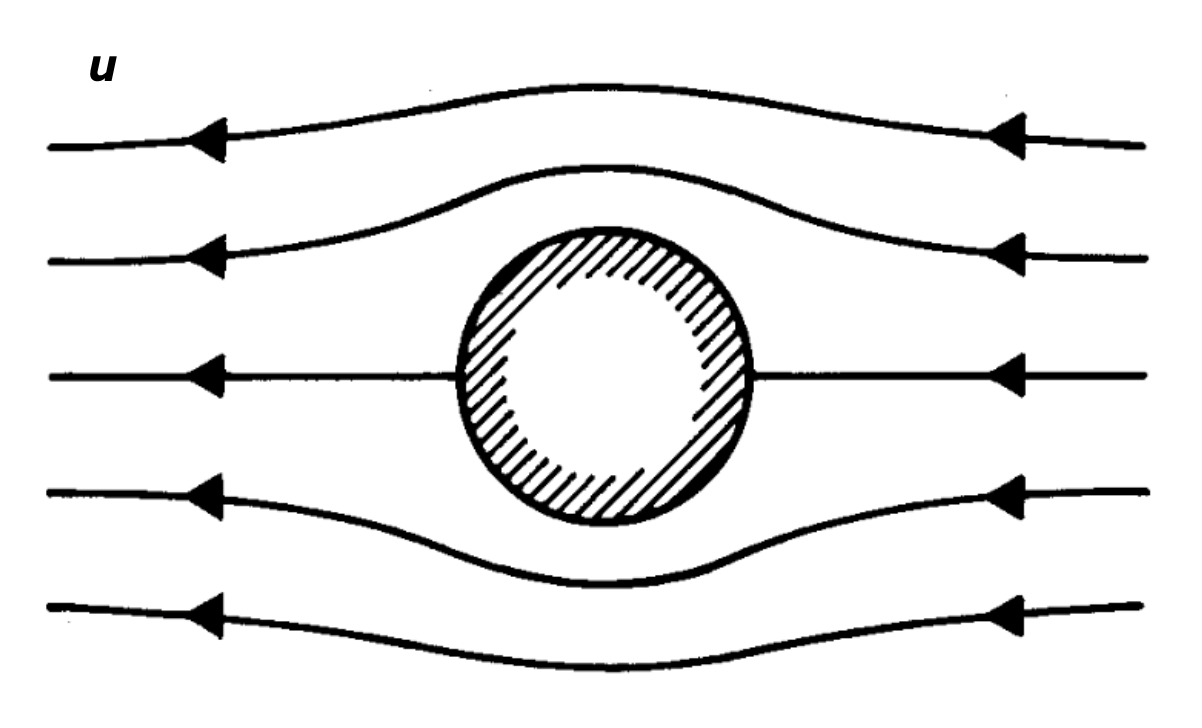
\includegraphics{./figs/DalembertParadox.png}}
  \end{center}
  \caption[]{D'Alembert paradox: a solid moving through an ideal fluid will
    experience no drag, contrary to everyday experience.}
  \label{fig:DalembertParadox}
\end{figure}

Let us find the force on cylinder moving through a
fluid at rest \figp{fig:DalembertParadox}. This is equivalent to a flow past an obstacle at
rest. The obstacle displaces an equal volume of fluid, of mass
$m$. This mass is flowing with velocity u, so its kinetic energy is
$mu^2/2$. The work done by the fluid on the obstable is the time
derivative of the kinetic energy 

\beq
\v{f}\cdot\v{u} =  \frac{dK}{dt} = \frac{m}{2}\frac{d}{dt}\v{u}\cdot\v{u} = m\v{u}\cdot\frac{d\v{u}}{dt}
\eeq

finding the force 

\beq
\v{f} = m\frac{d\v{u}}{dt}
\eeq

This is a curious result. In steady state, there is no force acting on the obstacle. This
goes against our everyday experience that a fluid exerts a drag
force on any object moving through it. This is $d'Alembert's
paradox$, established in 1752. 

This paradox arises because we have neglected viscosity in
our equations. If a body moving through a fluid were to be slowed
by a drag force, the kinetic energy lost in the slowing process has to
go somewhere. In a viscous fluid, it can go to heat. Since this is not
possible in an ideal fluid, we come up with the result that an ideal fluid
cannot exert drag on objects moving through it.

But we have considered that the flow has high Reynolds number. We can
ignore viscosity. What is the problem? 

\subsection{Boundary layers}

The solution to the paradox was found by Prandtl in 1904, a century after
D'Alembert established it.

\begin{figure}
  \begin{center}
    \resizebox{\textwidth}{!}{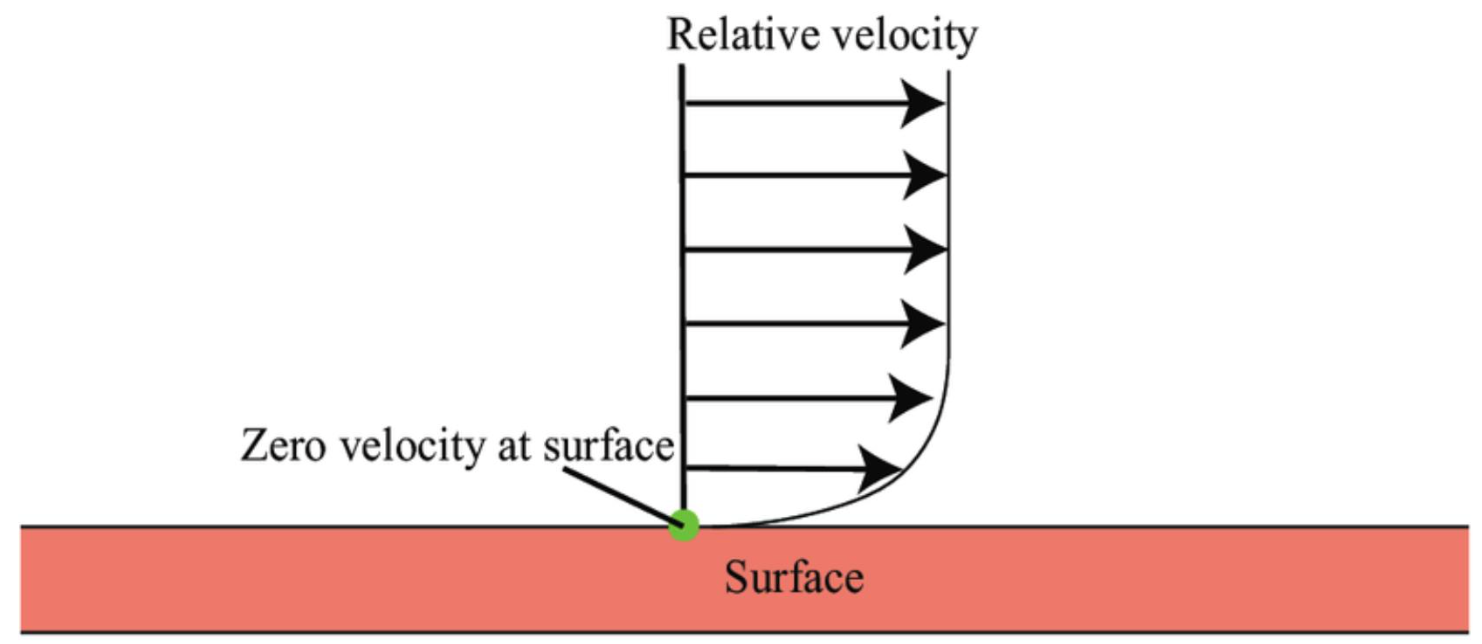
\includegraphics{./figs/noslip_condition.png}}
  \end{center}
  \caption[]{No-slip boundary condition: a fluid comes to rest at a surface.}
  \label{fig:noslip}
\end{figure}

The fluid at the boundary has zero velocity -- which is known as the {\it no-slip boundary
  condition} \figp{fig:noslip}. This leads to strong shear between the boundary at zero,
and the rest of the (moving) fluid. In this region, the shear makes
$\Laplace{\v{u}}$ so strong that viscosity cannot be ignored, even at high
Reynolds number. Essentially, the no-slip boundary condition becomes a
source of vorticity. The viscous term then diffuses the vortex into
the flow. 

\classcomm{Everyday observational experience: the seeing is produced inside the dome.}

Consider pipe flow. The flow is established by a pressure gradient,
and in equilibrium with the viscous force

\beq
\mu\Laplace{\v{u}}=\grad{p} 
\eeq

\noindent approximating $\grad{p}=\Delta p / L$ where $L$ is the length of the
pipe, and writing $\Laplace{\v{u}}$ in cylindrical coordinates 

\beq
\frac{1}{r}\frac{d}{dr}\left(r\frac{du}{dr}\right) =\frac{\Delta p}{\mu L} 
\eeq

\noindent with boundary conditions $u=0$ at $r=a$ (no slip condition), and
$du/dr=0$ at $r=0$ (so the flow is continuous).

\beq
\frac{d}{dr}\left(r\frac{du}{dr}\right) =\frac{\Delta p}{\mu L} r
\eeq

\noindent and integrating 

\beq
r\frac{du}{dr} =\frac{\Delta p}{2\mu L} r^2 + C_1
\eeq

\noindent dividing by $r$

\beq
\frac{du}{dr} =\frac{\Delta p}{2\mu L} r + \frac{C_1}{r}
\eeq

\noindent the Newman boundary condition at $r=0$ implies $C_1=0$. Integrating again

\beq
u(r) =\frac{\Delta p}{4\mu L} r^2 + C_2 
\eeq

\noindent and the Dirichlet boundary condition $u=0$ at $r=a$, implies 

\beq
u(r) =\frac{\Delta p}{4\mu L} \left(r^2 -a^2\right)
\eeq

\noindent so the flow is parabolic \figp{fig:pipe_flow}.

\begin{figure}
  \begin{center}
    \resizebox{\textwidth}{!}{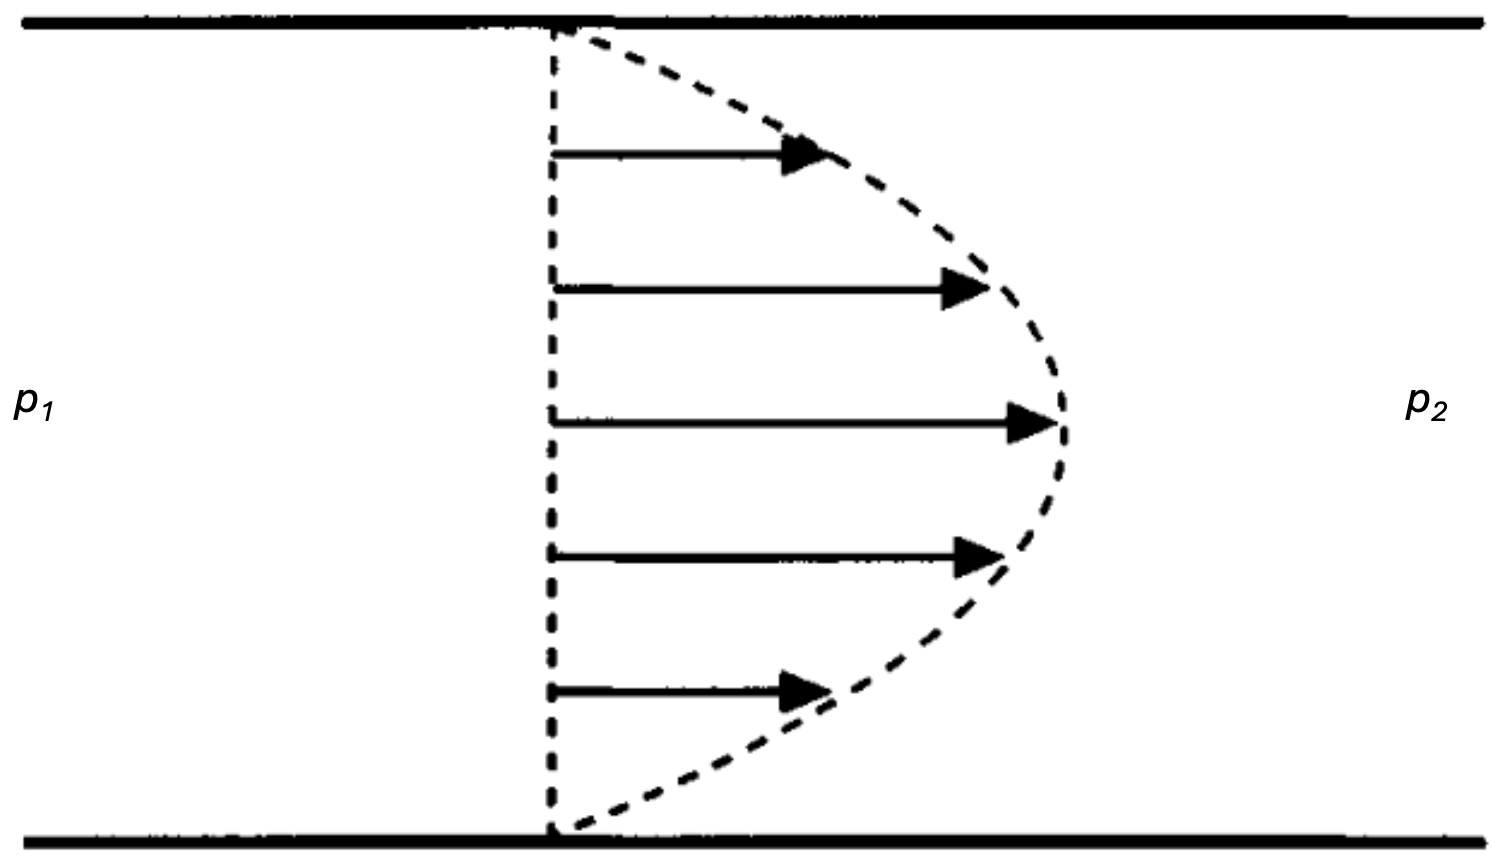
\includegraphics{./figs/pipe_flow.png}}
  \end{center}
  \caption[]{Pipe flow. The flow comes to rest at the boundary,
    assuming a parabolic shape.}
  \label{fig:pipe_flow}
\end{figure}


\subsection{Shear and flow past an obstacle}

Notice that this flow has vorticity. 

\beq
\omega = \frac{\partial u_x}{\partial y}
\eeq

A viscous flow can start with zero shear, and the no-slip
condition develops shear and vorticity. This is an important
qualitative concept to internalize: {\it a boundary is a vorticity
  source}. This is clearly illustrated in the von Karman vortex
street, one of the most iconic phenomena of fluid dynamics
\figp{fig:vonkarman}. Past the obstacle, the flow develops vortices of
opposite polarity in the flow downstream. 

\begin{figure}
  \begin{center}
    \resizebox{\textwidth}{!}{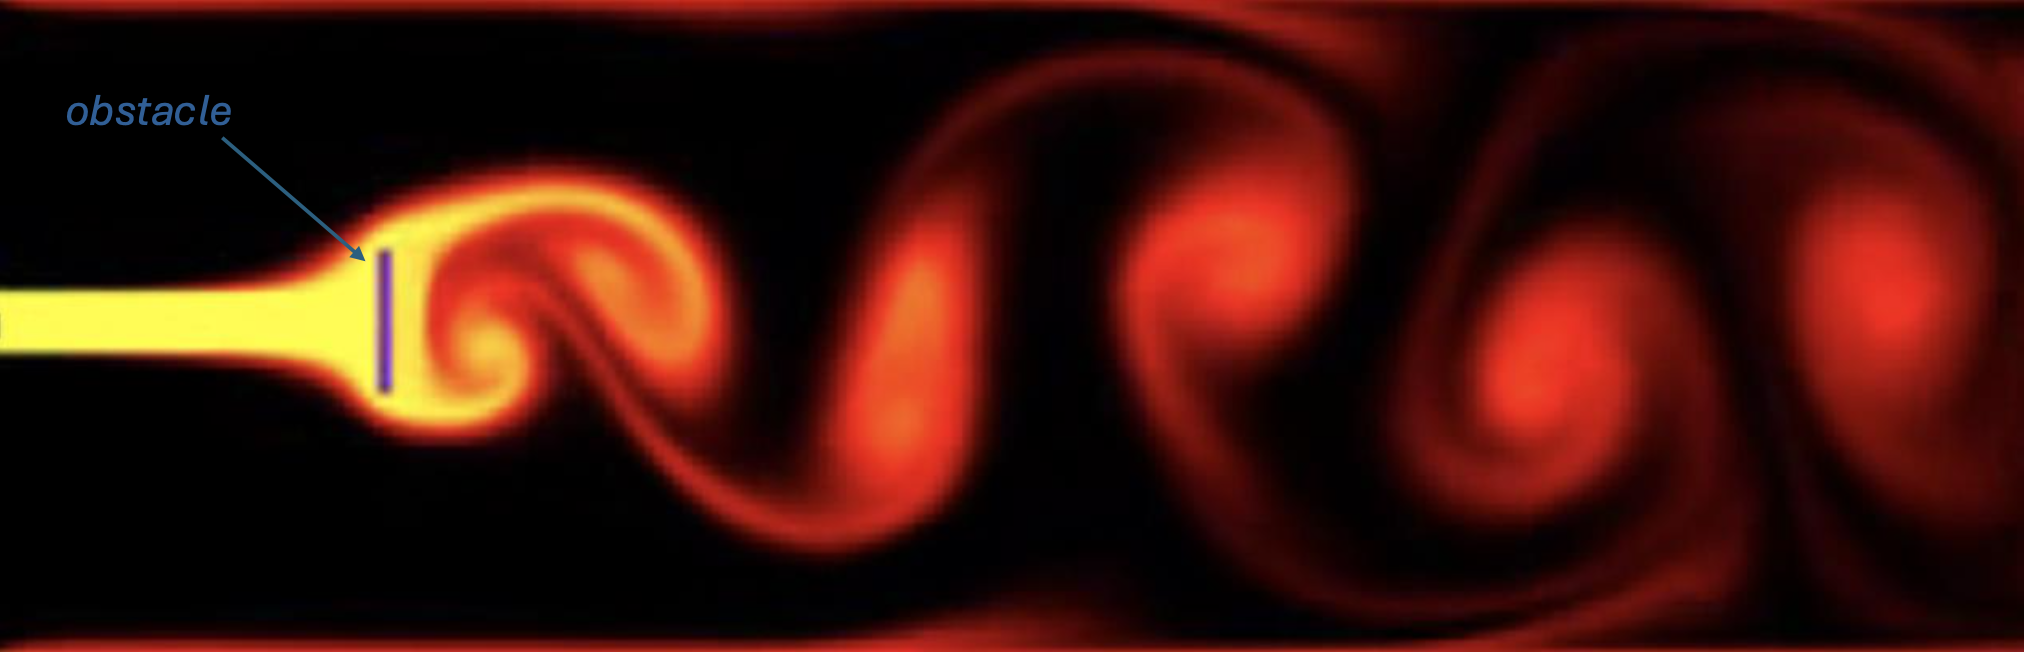
\includegraphics{./figs/VonKarmanStreet.png}}
  \end{center}
  \caption[]{von Karman vortex street in flow past an obstacle.}
  \label{fig:vonkarman}
\end{figure}


A familiar example is atmospheric seeing. A difference in seeing can be observed
in different sides of a mountain, for instance, the windward (upwind) will often
have better seeing than the leeward (downwind) direction. This is because the mountain itself
is an obstacle. A sketch of the flow is shown in \fig{fig:oceanmountain}

\begin{figure}
  \begin{center}
    \resizebox{\textwidth}{!}{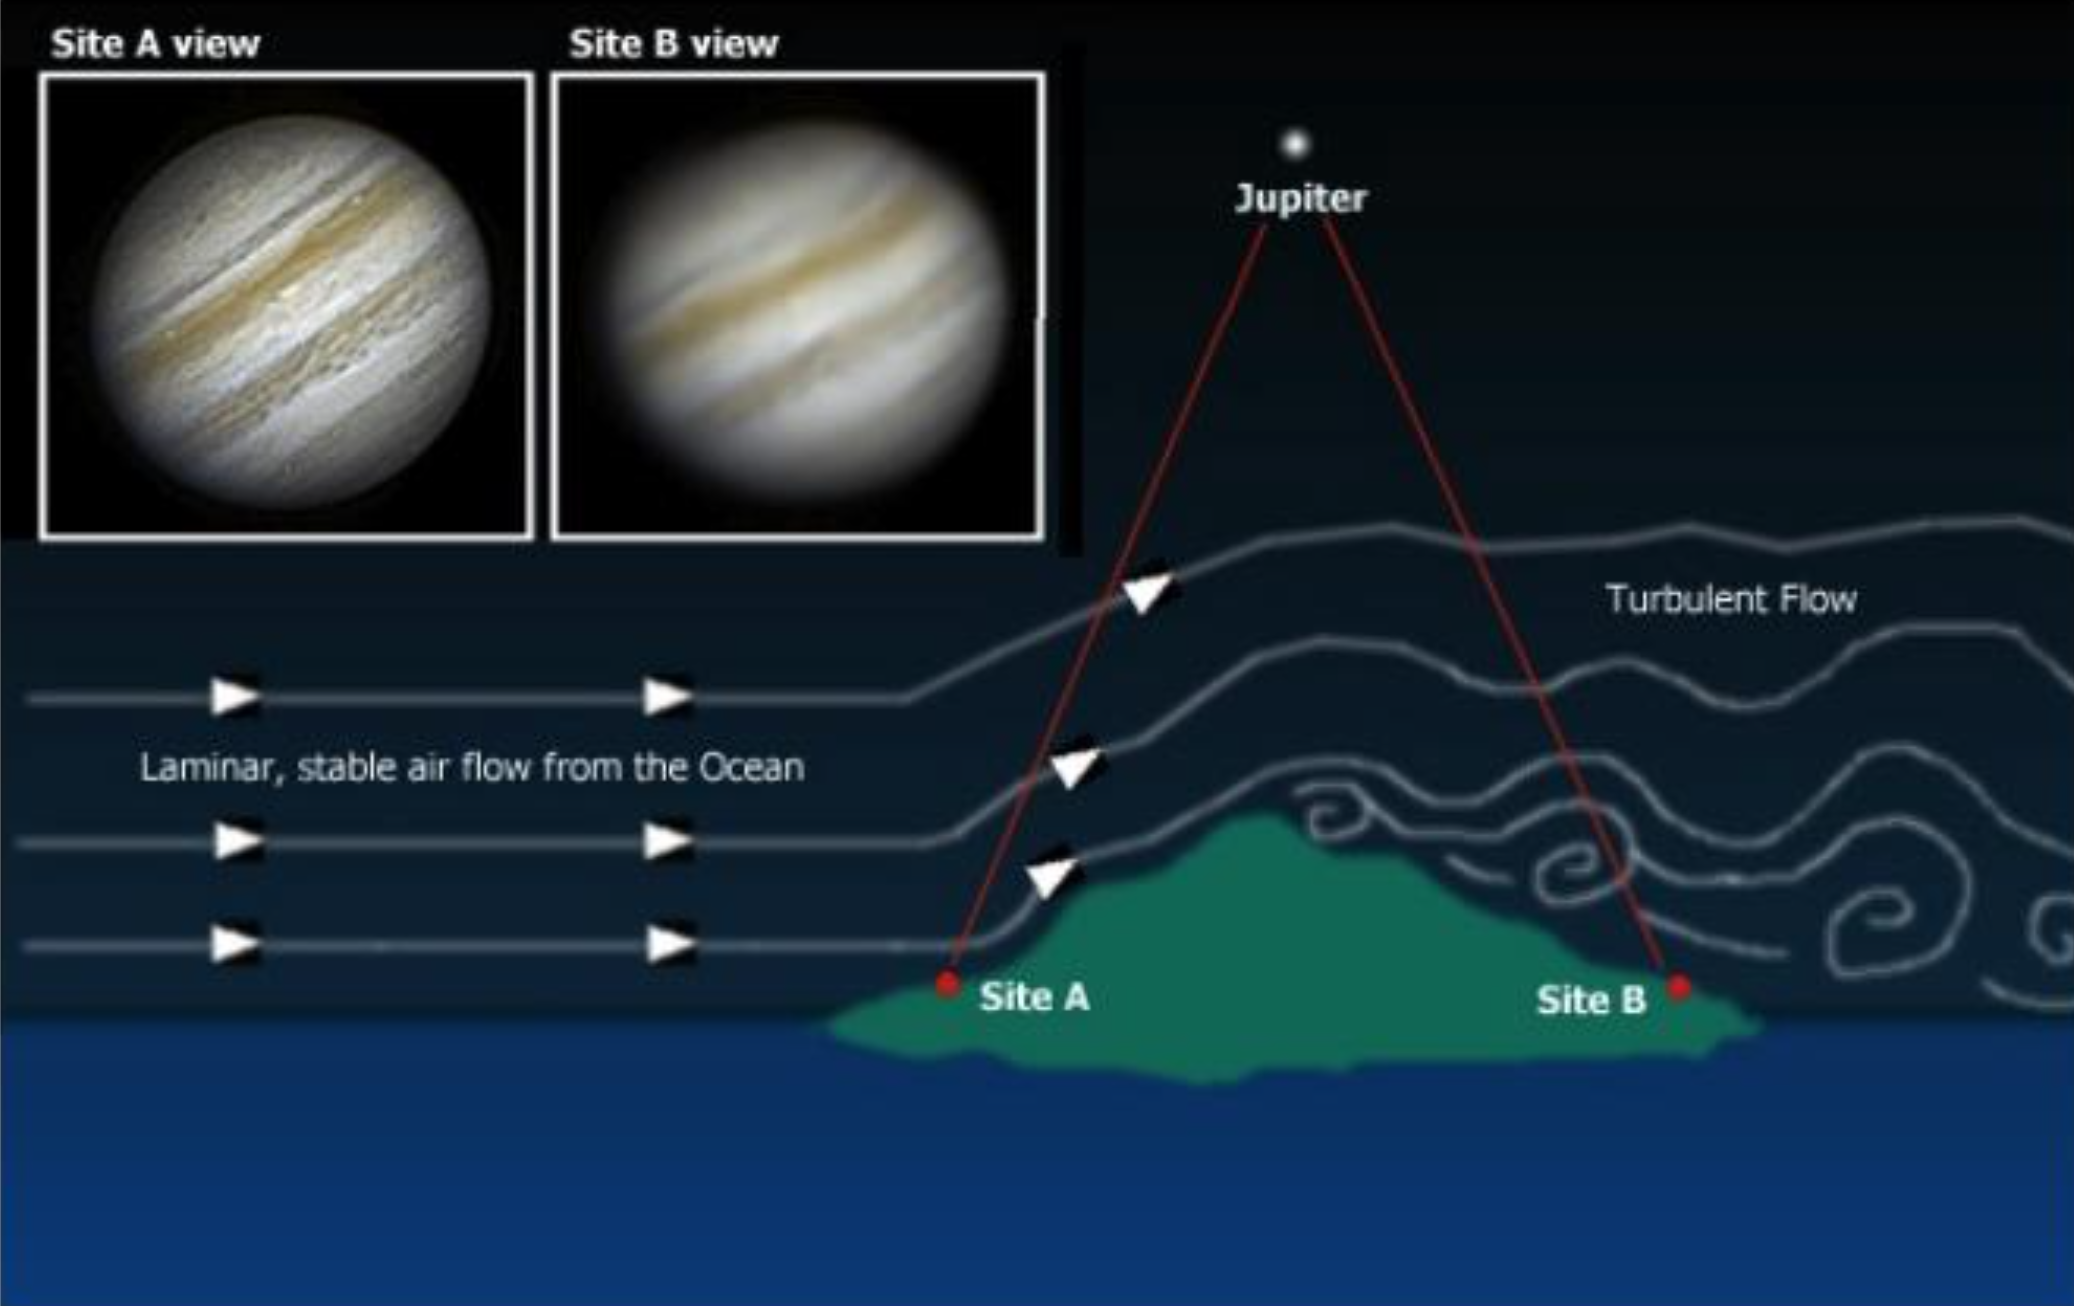
\includegraphics{./figs/flowpastmountain.png}}
  \end{center}
  \caption[]{Turbulent wake in flow past an island. The seeing upwind is usually better than the seeing downwind.}
  \label{fig:oceanmountain}
\end{figure}


But how is the shear developed at the boundary layer converted into
vorticity? We will tackle that when studying Kelvin-Helmholtz and
Rayleigh-Taylor instabilities. For now, let us notice that {\it shear and
vorticity have the same dimension}. The definition of the shear tensor is

\beq
S_{ij} = \frac{1}{2}\frac{\partial u_i}{\partial x_j} + \frac{\partial u_j}{\partial x_i} 
\eeq

\noindent whereas the rotation tensor is 

\beq
\Omega_{ij} = \frac{1}{2}\frac{\partial u_i}{\partial x_j} - \frac{\partial u_j}{\partial x_i} 
\eeq

The vorticity is defined as

\beq
\Omega_{ij}=-\frac{1}{2}\varepsilon_{ijk}\omega_k
\eeq

\noindent shear and vorticity are two sides of the same coin. 

\section{Rotating frames}


\begin{figure}
  \begin{center}
    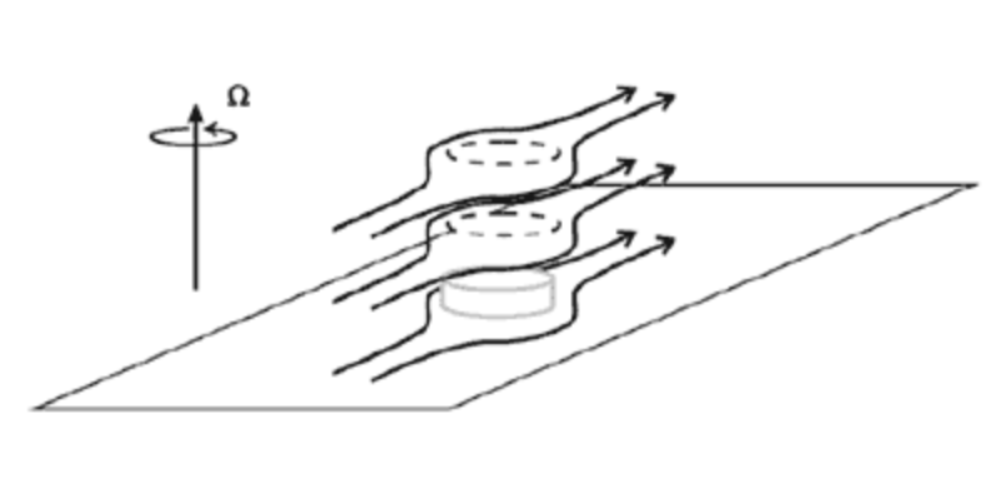
\includegraphics[height=.35\linewidth]{./figs/tp1.png}
    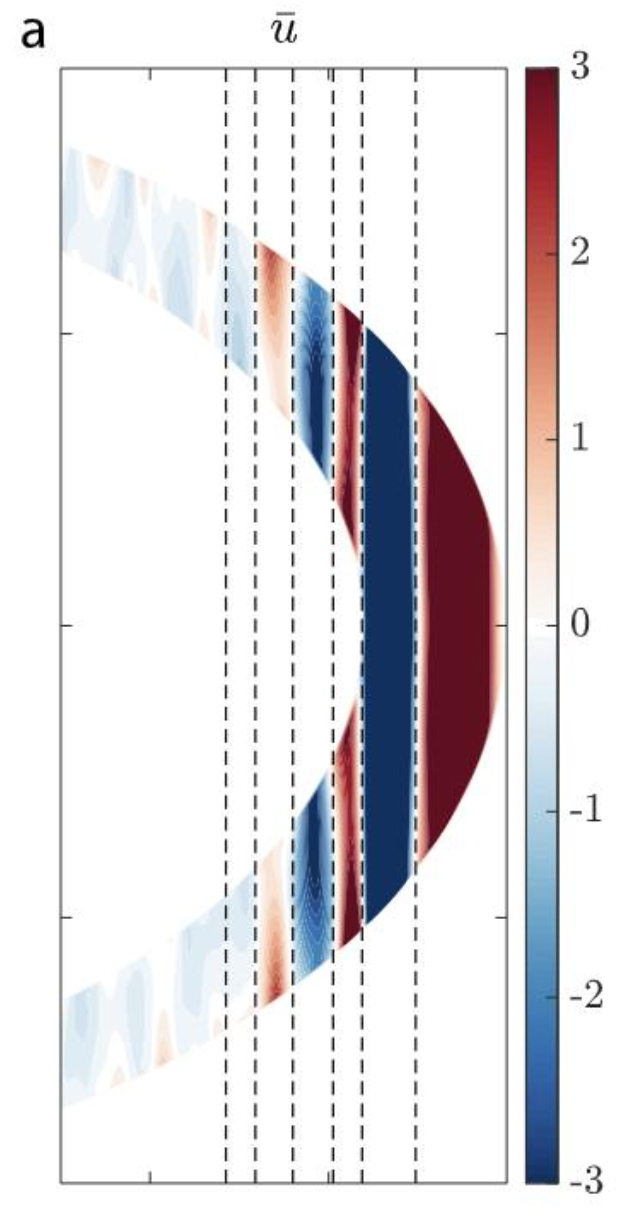
\includegraphics[height=.45\linewidth]{./figs/tp2.png} 
  \end{center}
  \caption[]{Left: The Taylor-Proudmann theorem demands that vertical
    columns of fluid move along contours of constant fluid depth. Thus
    fluid columns act as if they were rigid and move along contours of
    constant fluid depth. Horizontal flow is thus deflected as if the
    obstacle extedned through the whole depth of the fluid. Right:
    Interior model of Jupiter showing how a fast rotator shows a flow
    pattern constant in cylinders along the rotation axis.}
  \label{fig:taylor-proudmann}
\end{figure}

In astrophysics it is often useful to work in a frame rotating with constant
angular speed $\v{\Omega}$. This may be the frame in which a binary system is
stationary, a rotating fluid is at rest, or a spiral pattern is stationary. In
a rotating frame, we simply add the Coriolis and centrifugal forces to
the RHS of the Euler equation, which gives the forces acting on fluid
elements, just as we would do for Newtonian point-particle mechanics.
Thus the Euler equation in a rotating frame is

\beq
\ptderiv{\v{u}} +\left(\v{u}\cdot  \grad\right) \v{u} =
-\frac{1}{\rho}\grad{p}  - 2\v{\Omega}\times\v{u} - \v{\Omega}\times\v{\Omega}\times\v{r}
\eeq

and the velocity measured in the inertial frame is

\beq
\v{u}_{\rm inertial} = \v{u} + \v{\Omega}\times\v{r}
\eeq

\subsection{Taylor-Proudman theorem}

If the centrifugal force can be neglected, a steady state flow will be
in equilibrium between the pressure gradient and the Coriolis
force. Such a flow is called {\it geostrophic} flow

\beq
2\v{\Omega}\times\v{u} = -\frac{1}{\rho}\grad{p} 
\eeq

\noindent taking the curl eliminates the pressure gradient, leading to 

\beq
\curl{\left(\v{\Omega}\times\v{u}\right)}  = 0 
\eeq

\noindent in index notation, the LHS is 

\beqn
\varepsilon_{ijk}\partial_j\varepsilon_{kpq}\Omega_p u_q &=&
\left(\delta_{ip}\delta_{jq}-\delta_{iq}\delta_{jp}\right) \partial_j
\Omega_p u_q\\
&=&\Omega_i\partial_j u_j - \Omega_j\partial_ju_i\\
\eeqn

\noindent where we considered $\v{\Omega}$ to be constant. If the flow is
imcompressible,

\beq
\left(\v{\Omega}\cdot\del\right)\v{u}=0
\eeq

Without loss of generality, we can
choose the axis $z$ to align with $\v{\Omega}$. In this case, the
theorem reduces to

\beq
\frac{\partial\v{u}}{\partial z} = 0 
\eeq

This remarkable theorem says that the flow is constant in cylinders:
symmetric around the rotation axis \figp{fig:taylor-proudmann}.


\begin{figure}
  \begin{center}
    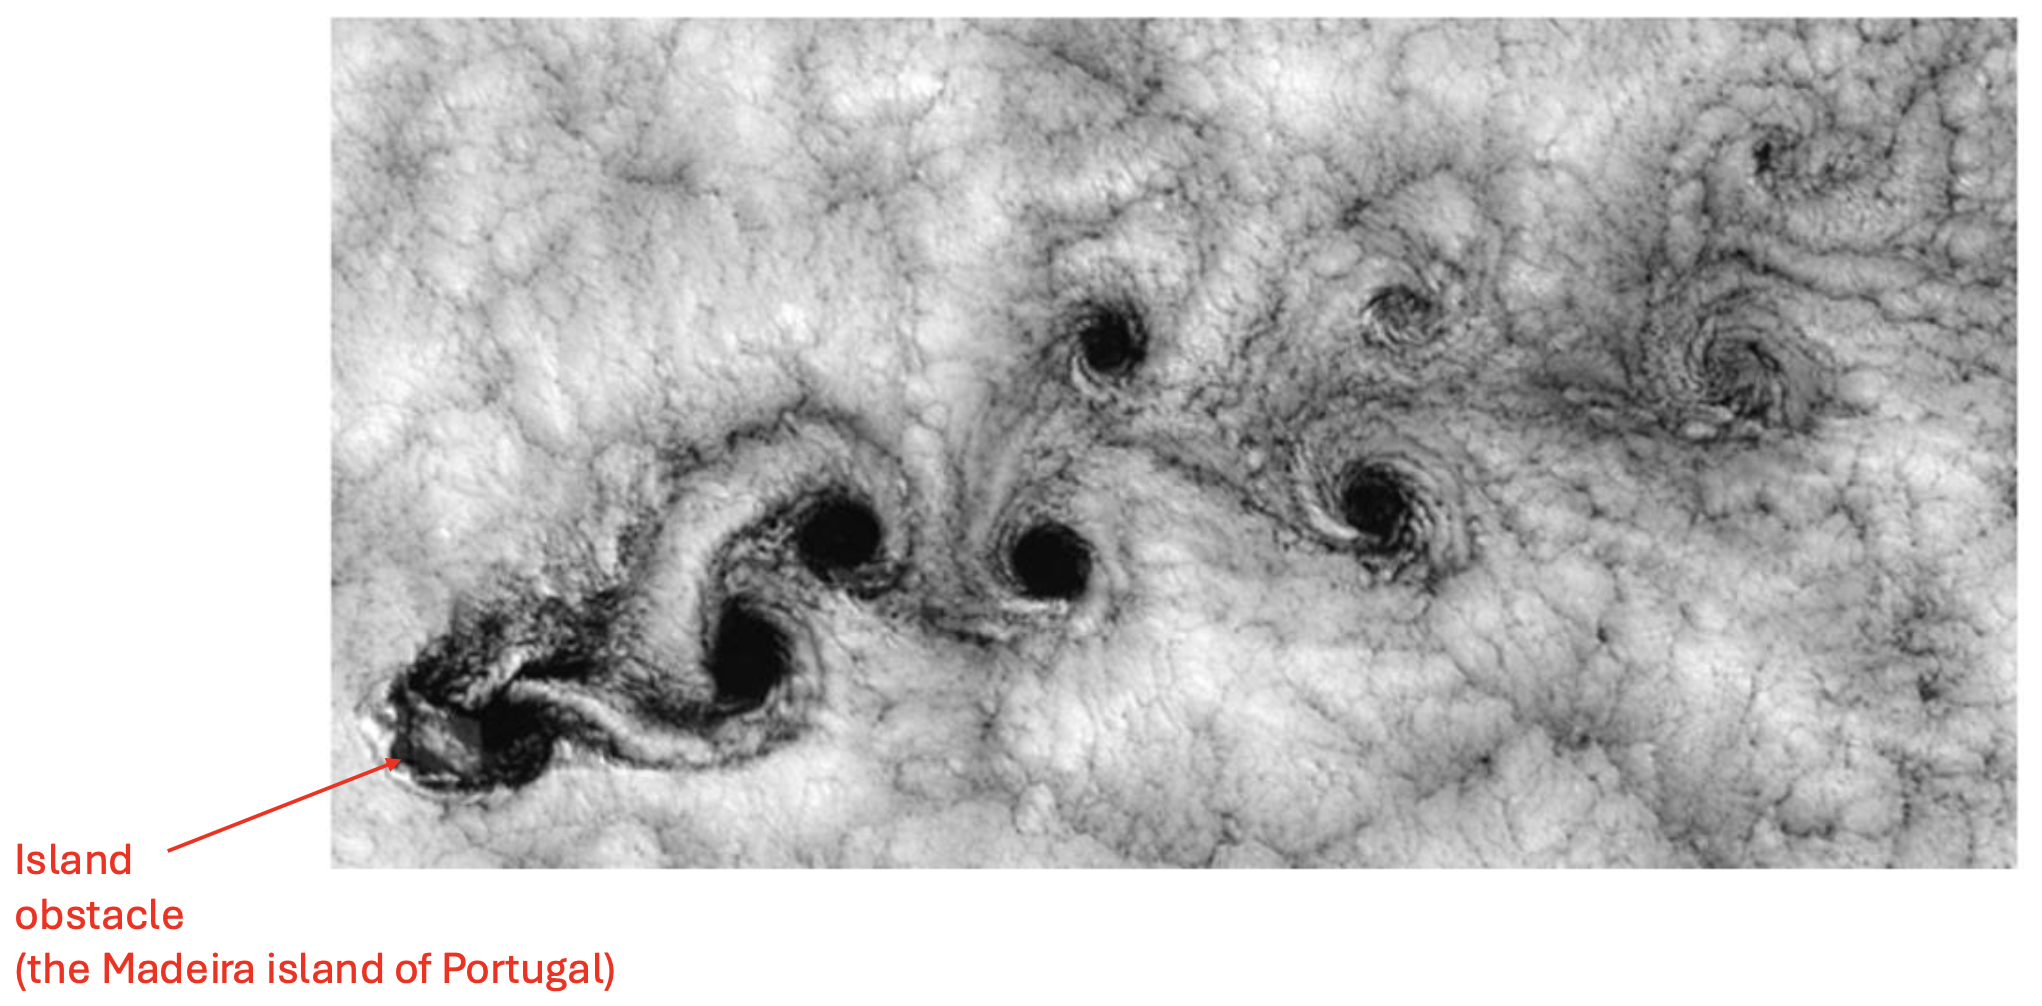
\includegraphics[width=\linewidth]{./figs/madeira.png}
  \end{center}
  \caption[]{Vortex street over Madeira island, the obstacle is the column of air over the island,
    which behaves like a Taylor column.}
  \label{fig:madeira}
\end{figure}


A phantasmagoric consequence of the Taylor-Proudman theorem is the {\it Taylor column}. A short obstacle at
{\it any} depth will produce a diversion of the flow at {\it all} depths. Because the fluid has to
rotate in cylinders, an obstacle diverting the flow at the bottom of a column \figp{fig:taylor-proudmann}
will make the whole column of fluid above it behave like an obstacle. This is the Taylor column.
The Taylor-Proudman theorem demands that vertical columns of fluid move along contours of constant fluid depth.
This fluid columns act as if they were rigid and move along contours of constant fluid depth. Horizontal flow
is thus deflected as if the obstacle extended through the whole depth of the fluid.
Notice in \fig{fig:madeira} the vortex street visible in the cloud deck. This vortex street is caused by
the island visible on the bottom left. The island is at sea level. The vortex street exists above
the island because there is a Taylor column above it.







